%%%%%%%%%%%%%%%%%%%%%%%%%%%%%%%%%%%%%%
%%%%%%%%%%%%%%%%%%%%%%%%%%%%%%%%%%%%%%
% Do not edit the TeX file your work
% will be overwritten.  Edit the RnW
% file instead.
%%%%%%%%%%%%%%%%%%%%%%%%%%%%%%%%%%%%%%
%%%%%%%%%%%%%%%%%%%%%%%%%%%%%%%%%%%%%%





\newcommand{\DefineMacros}{
\newcommand{\AlexNSur}{4,364}
\newcommand{\AlexNTar}{4,085,282}
\newcommand{\AlexSurmean}{0.462}
\newcommand{\AlexMrp}{0.288}
\newcommand{\AlexMrpSD}{0.0169}
\newcommand{\AlexRaking}{0.263}
\newcommand{\RefitTimeHours}{28}
\newcommand{\MrPawTimeSecs}{27}

}

%%%%%%%%%%%%%%%%%%%%%%
% Plots


\newcommand{\AlexanderImbalancePrimary}{

\begin{knitrout}
\definecolor{shadecolor}{rgb}{0.969, 0.969, 0.969}\color{fgcolor}\begin{figure}[!h]

{\centering 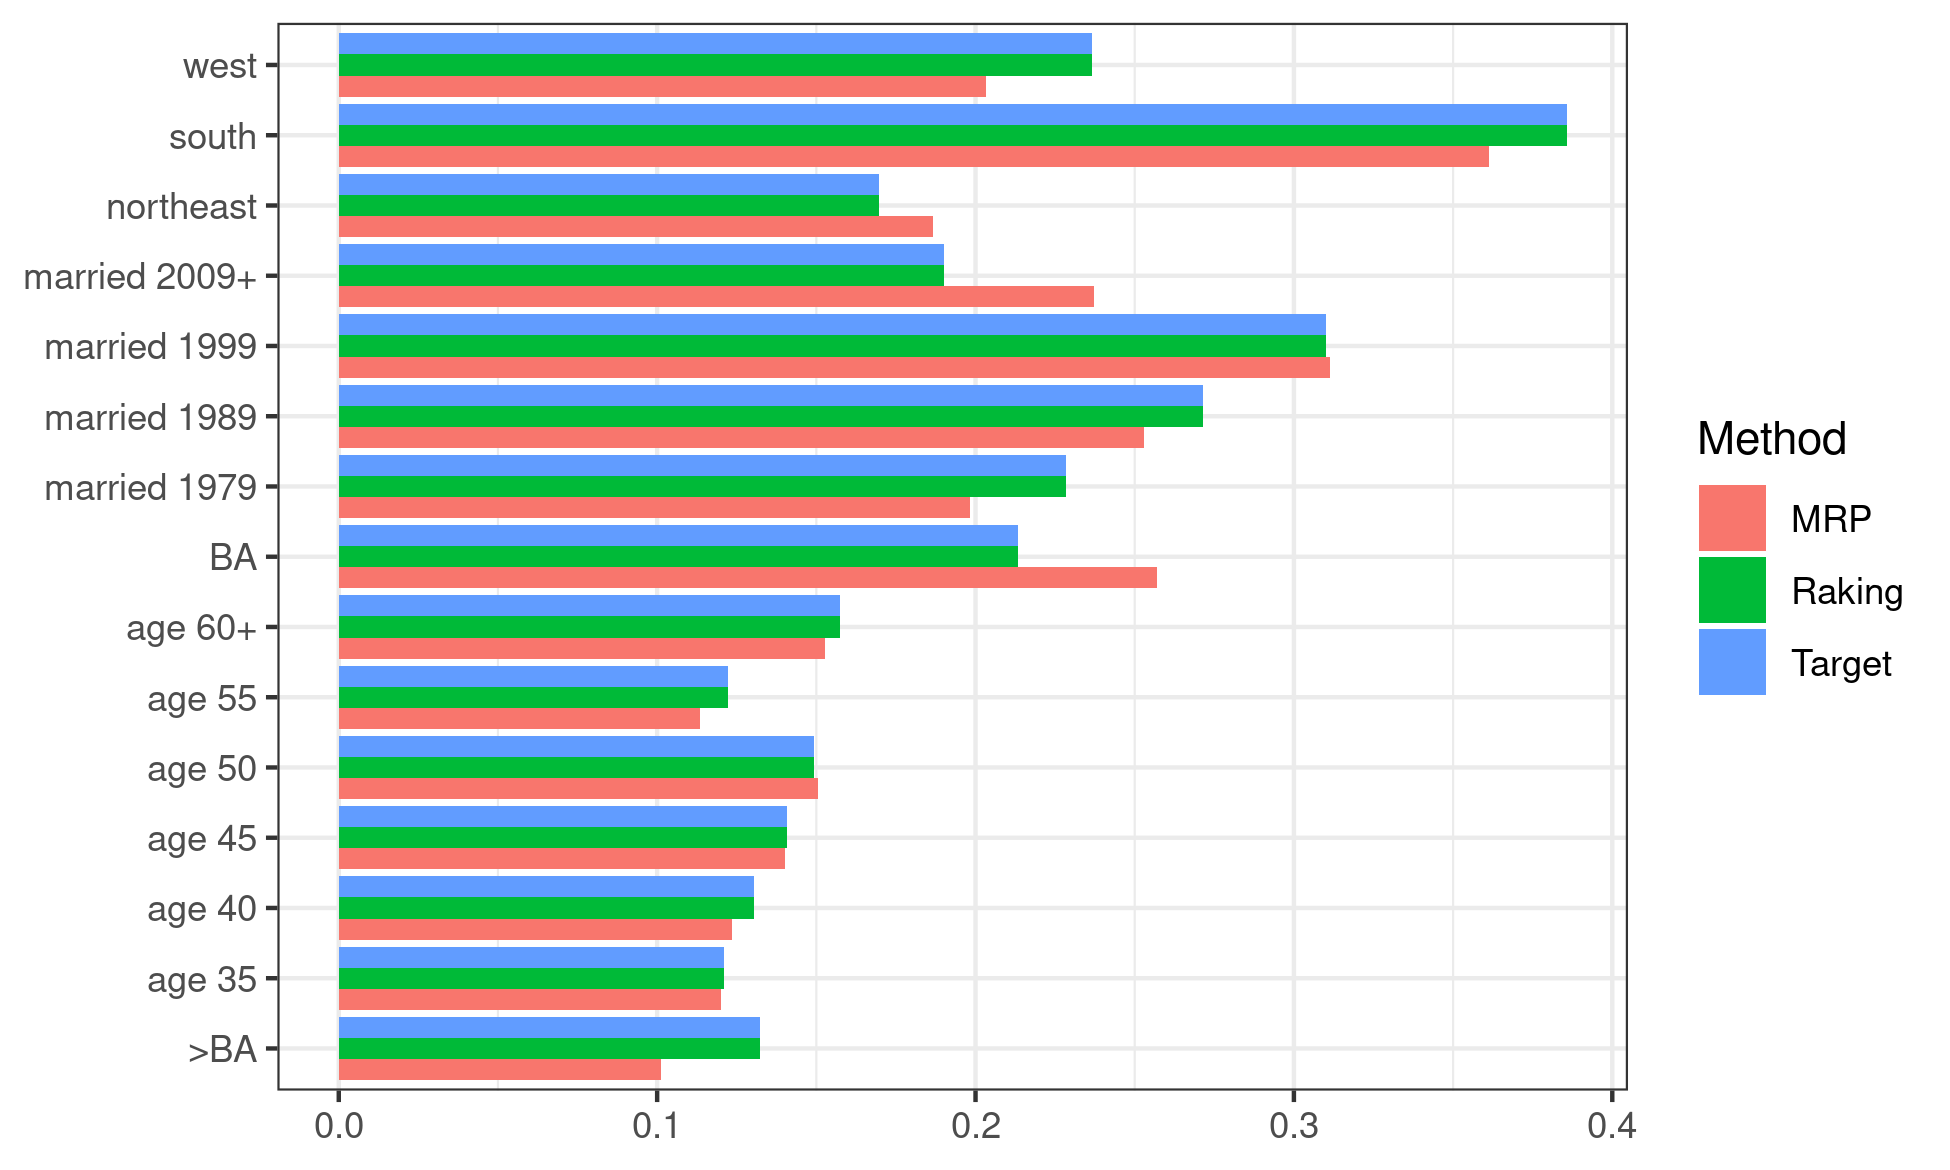
\includegraphics[width=0.98\linewidth,height=0.588\linewidth]{figure/alexanderprimary-1} 

}

\caption[Imbalance plot for primary effects]{Imbalance plot for primary effects}\label{fig:alexanderprimary}
\end{figure}

\end{knitrout}
}


\newcommand{\AlexanderImbalanceInteraction}{

\begin{knitrout}
\definecolor{shadecolor}{rgb}{0.969, 0.969, 0.969}\color{fgcolor}\begin{figure}[!h]

{\centering 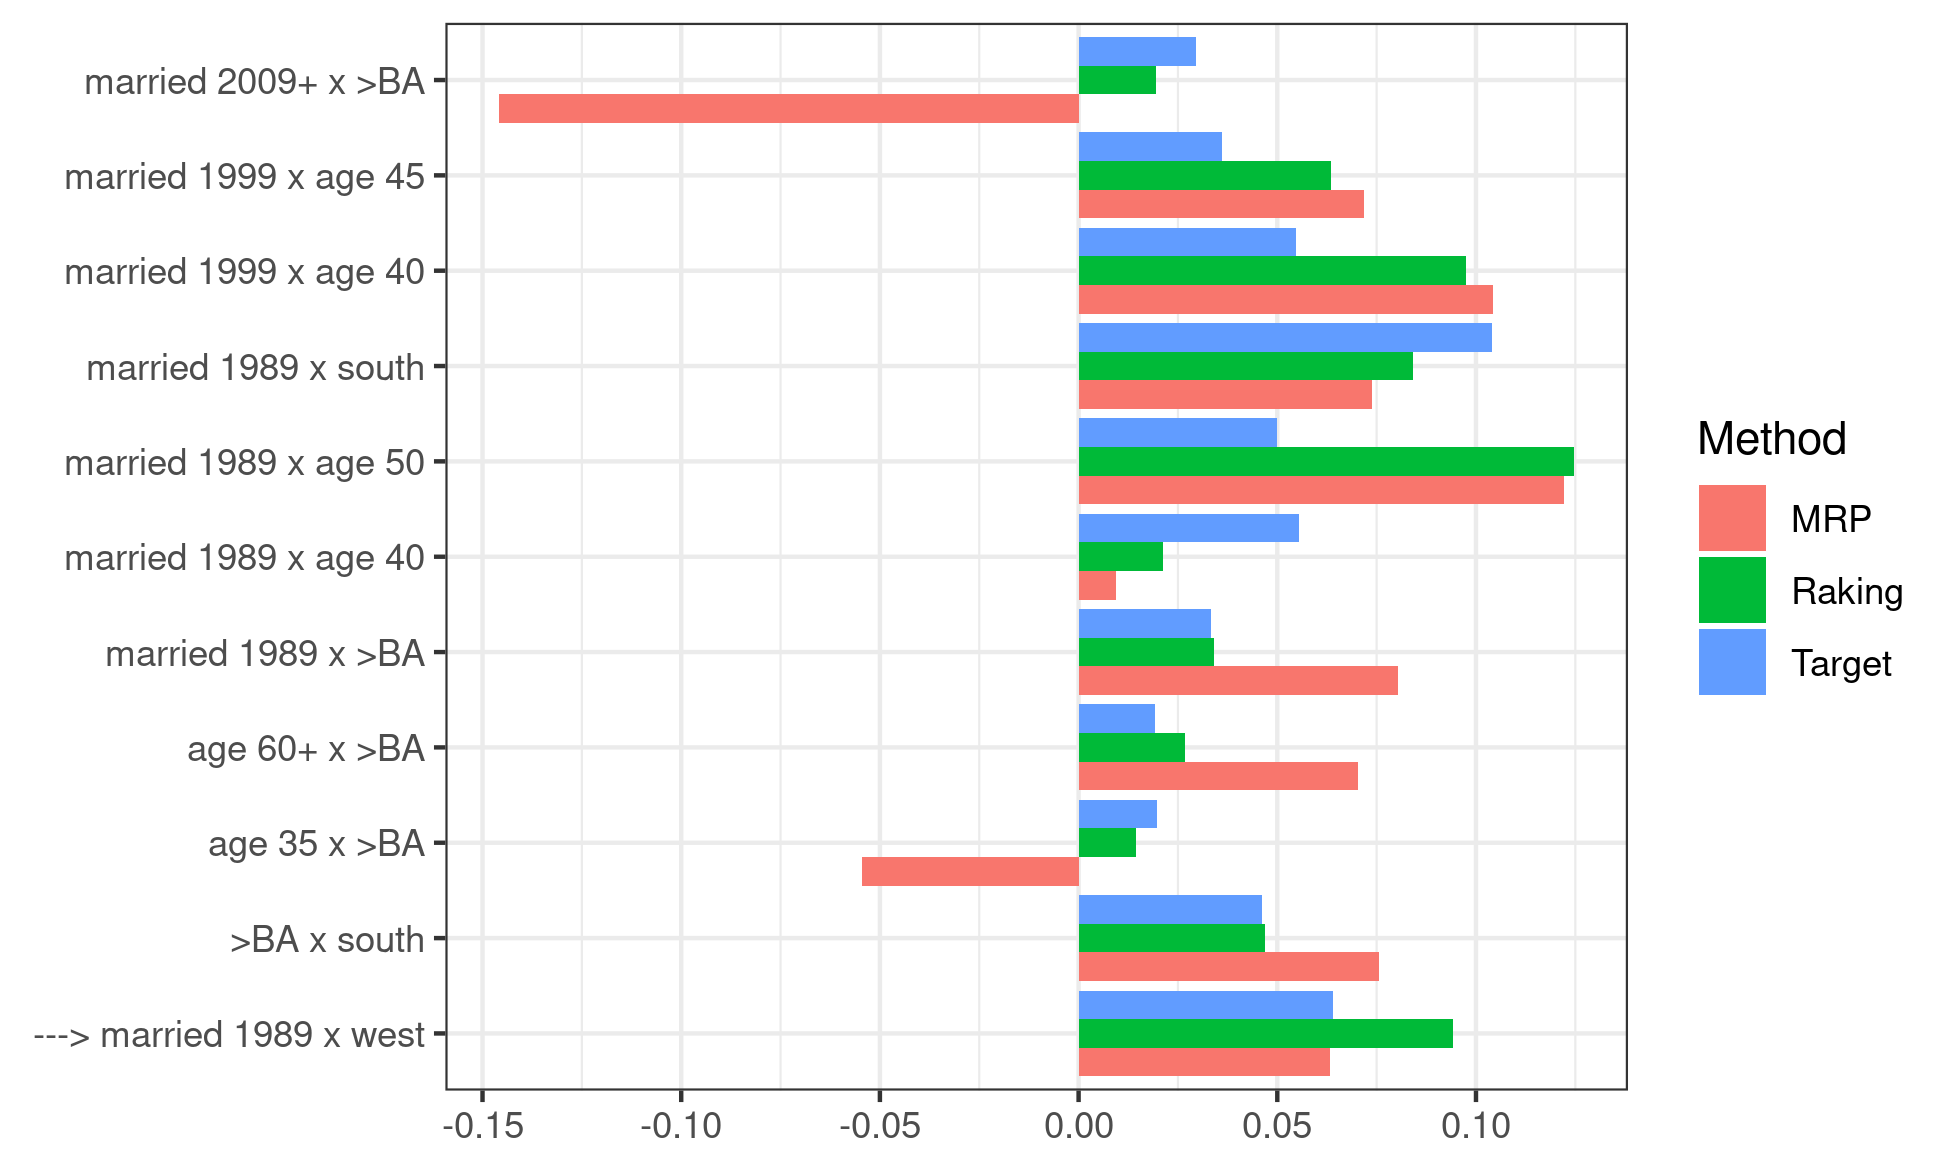
\includegraphics[width=0.98\linewidth,height=0.588\linewidth]{figure/alexanderinteraction-1} 

}

\caption[Imbalance plot for select interaction effects]{Imbalance plot for select interaction effects}\label{fig:alexanderinteraction}
\end{figure}

\end{knitrout}
}


\newcommand{\AlexanderPredictionInit}{

}


% Define the prediction graphs



\newcommand{\AlexanderPredictionFig}{

\begin{knitrout}
\definecolor{shadecolor}{rgb}{0.969, 0.969, 0.969}\color{fgcolor}\begin{figure}[!h]

{\centering 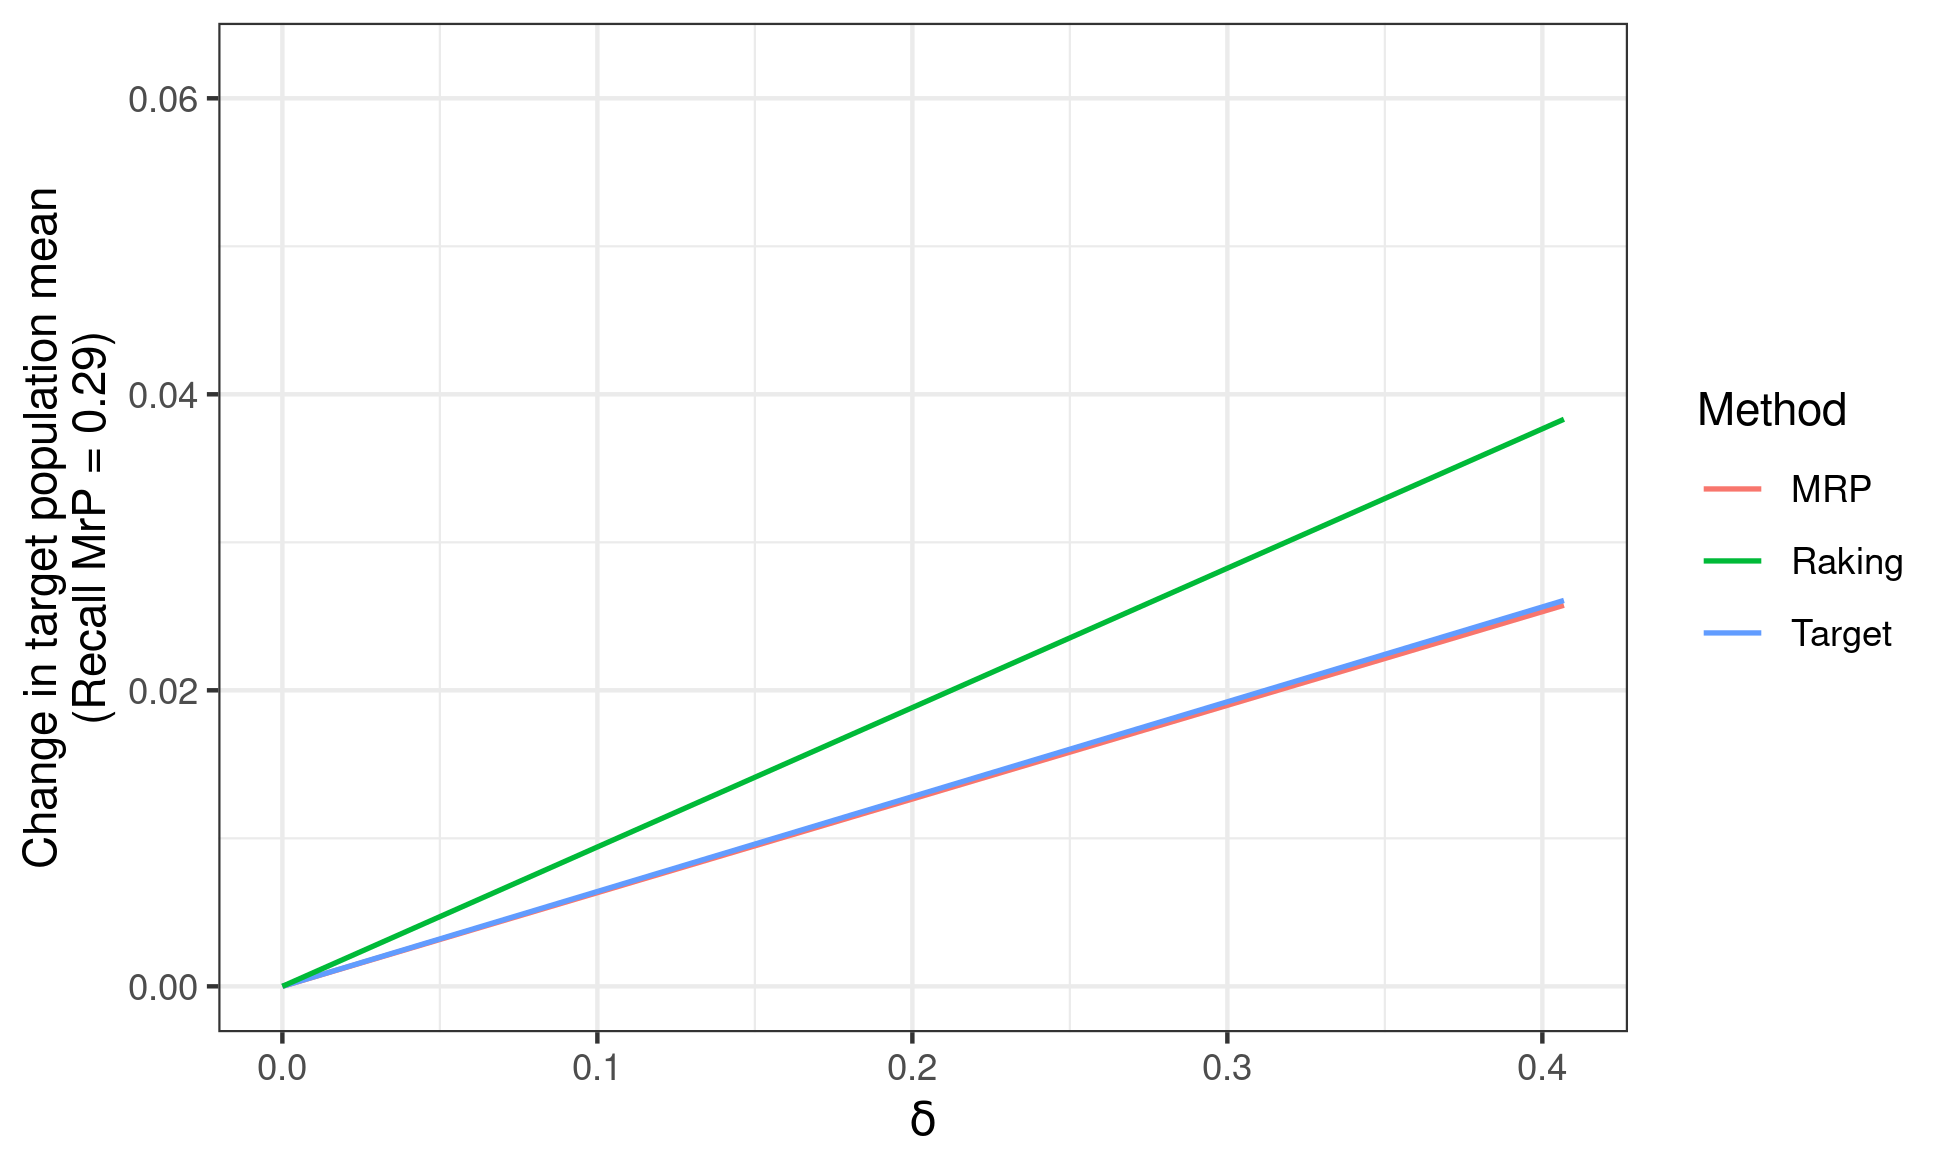
\includegraphics[width=0.98\linewidth,height=0.588\linewidth]{figure/alexandercontpred-1} 

}

\caption[Continuous predictions Alexander]{Continuous predictions Alexander}\label{fig:alexandercontpred}
\end{figure}

\end{knitrout}
}



\newcommand{\AlexanderPredictionFigTwo}{

\begin{knitrout}
\definecolor{shadecolor}{rgb}{0.969, 0.969, 0.969}\color{fgcolor}\begin{figure}[!h]

{\centering 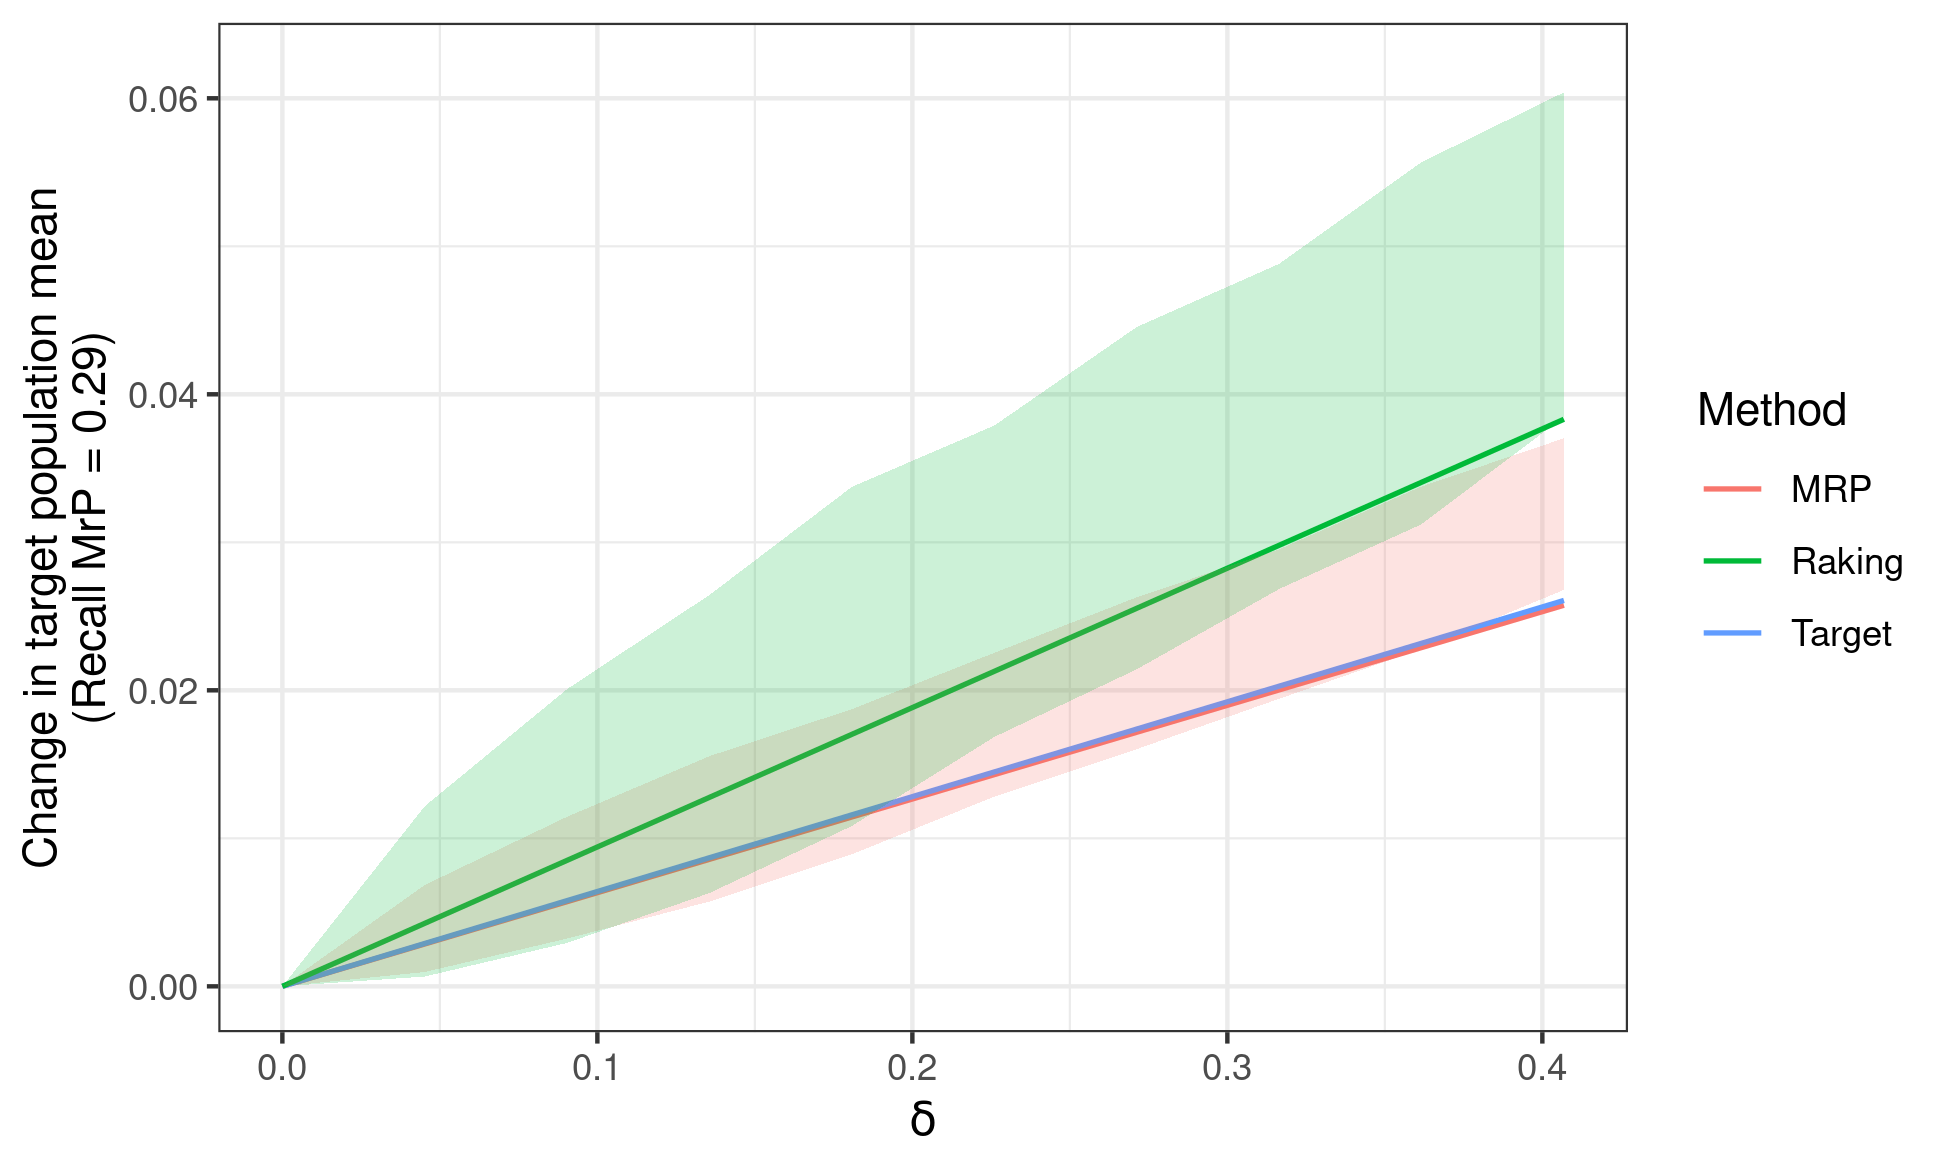
\includegraphics[width=0.98\linewidth,height=0.588\linewidth]{figure/alexanderdiscretepred-1} 

}

\caption[Continuous predictions Alexander]{Continuous predictions Alexander}\label{fig:alexanderdiscretepred}
\end{figure}

\end{knitrout}
}



\newcommand{\AlexanderPredictionFigThree}{

\begin{knitrout}
\definecolor{shadecolor}{rgb}{0.969, 0.969, 0.969}\color{fgcolor}\begin{figure}[!h]

{\centering 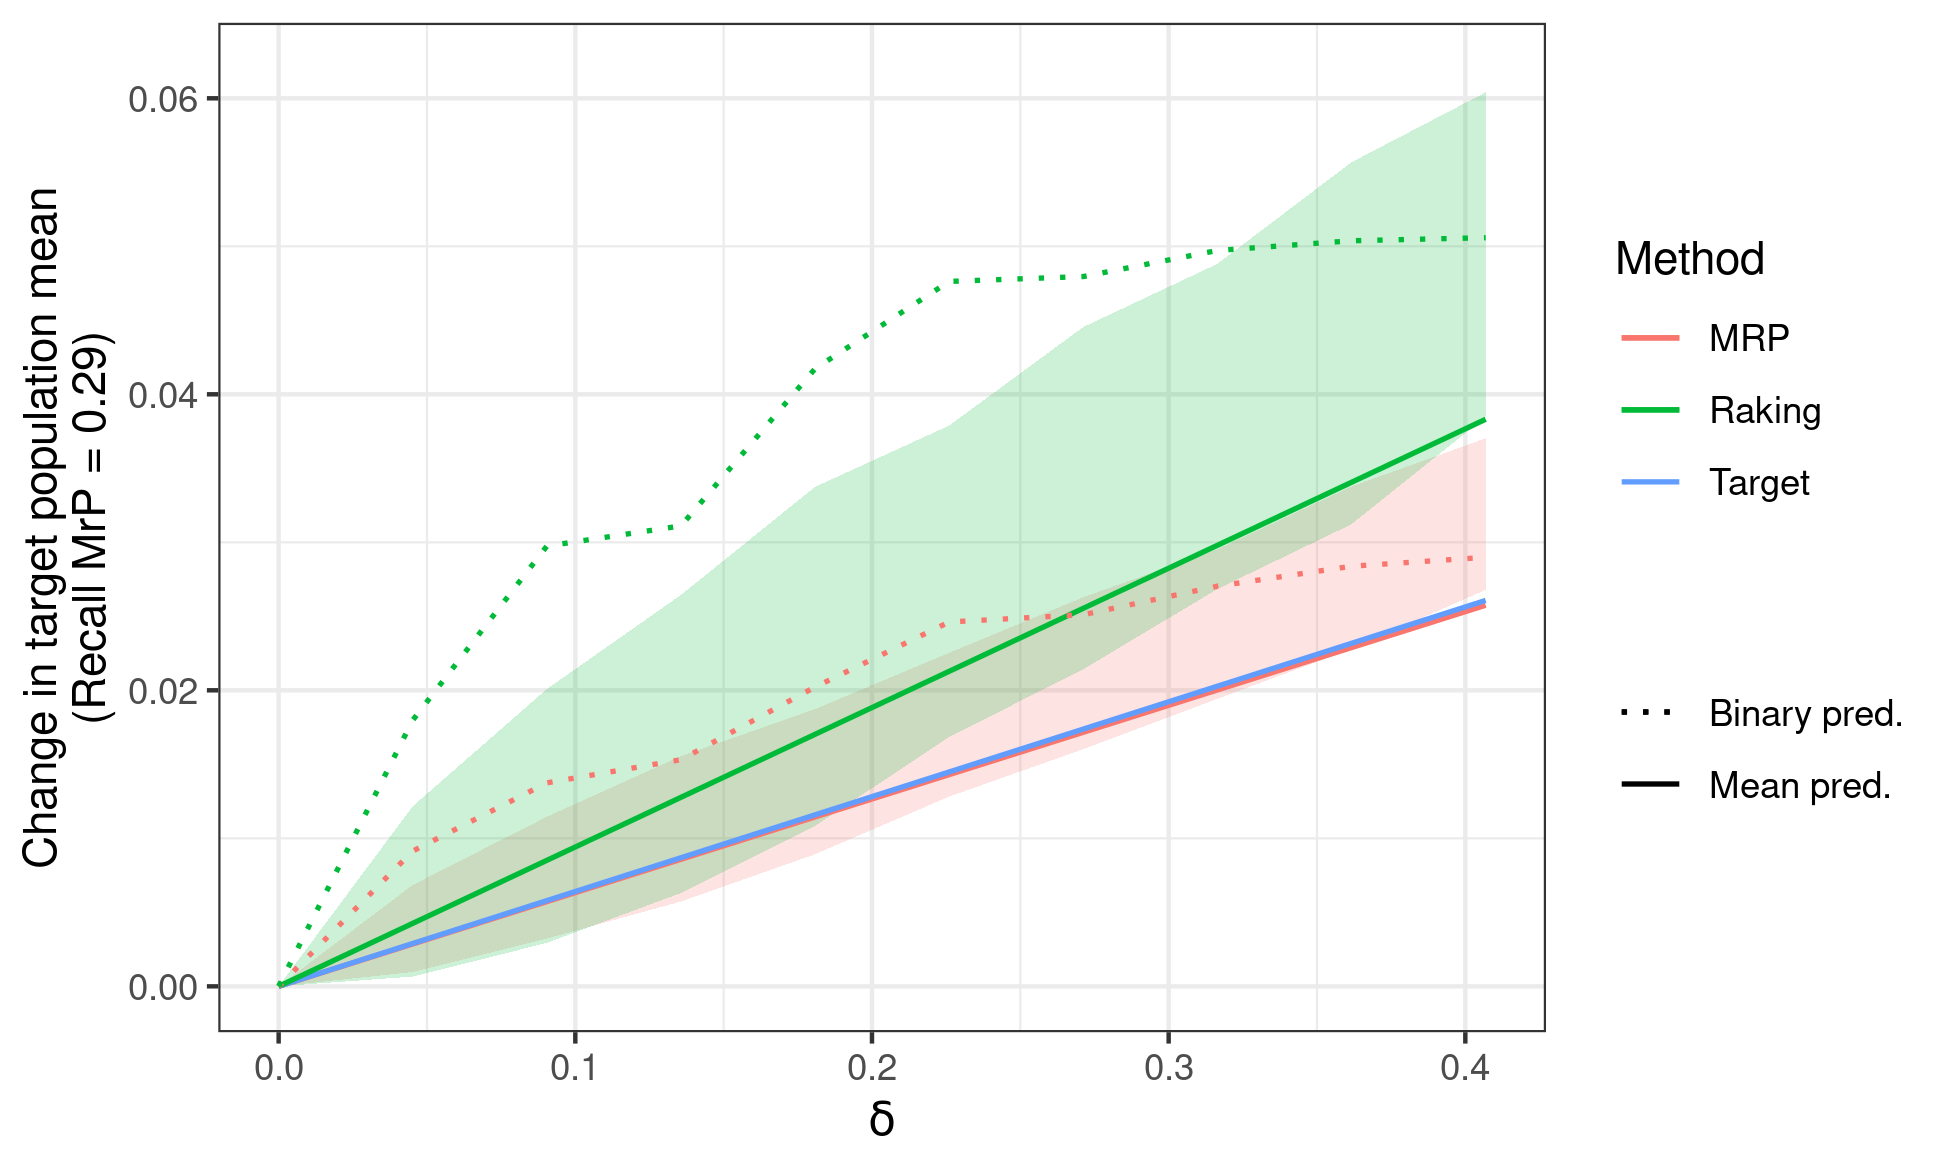
\includegraphics[width=0.98\linewidth,height=0.588\linewidth]{figure/alexanderbinarypred-1} 

}

\caption[Continuous predictions Alexander]{Continuous predictions Alexander}\label{fig:alexanderbinarypred}
\end{figure}

\end{knitrout}
}




\newcommand{\AlexanderPredictionFigFour}{

\begin{knitrout}
\definecolor{shadecolor}{rgb}{0.969, 0.969, 0.969}\color{fgcolor}\begin{figure}[!h]

{\centering 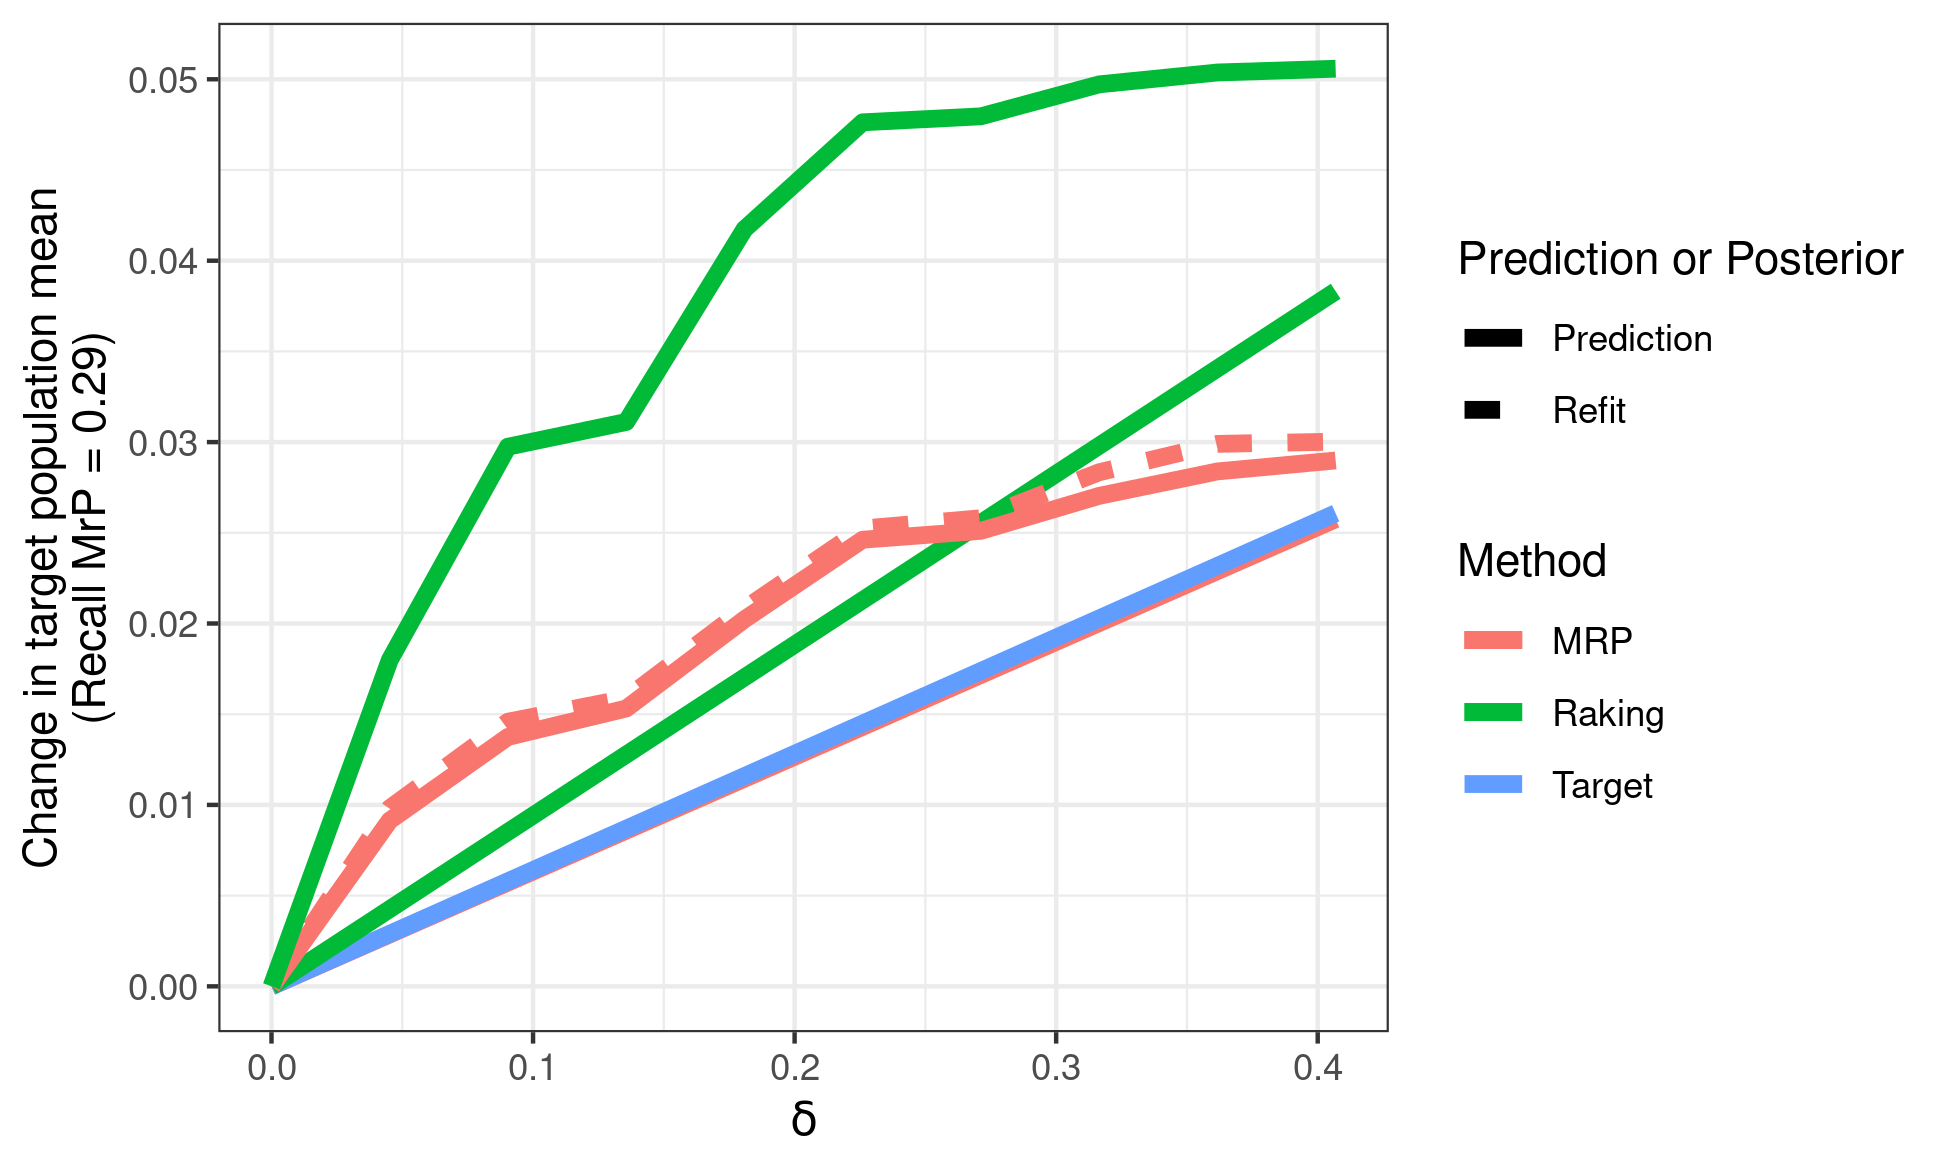
\includegraphics[width=0.98\linewidth,height=0.588\linewidth]{figure/alexanderrefit-1} 

}

\caption[Continuous predictions Alexander]{Continuous predictions Alexander}\label{fig:alexanderrefit}
\end{figure}

\end{knitrout}
}
